\documentclass[11pt,a4paper]{article}
\usepackage[margin=2.3cm]{geometry}
\usepackage[T1]{fontenc}
\usepackage[utf8]{inputenc}
\usepackage{lmodern}
\usepackage{amsmath,amssymb,bm,mathtools}
\usepackage{booktabs,graphicx,microtype}
\usepackage[hidelinks]{hyperref}
\hypersetup{pdftitle={Surface field transport and direction-resolved Fresnel transmission in a Q inverse T Q optical pipeline},pdfsubject={Manuscript draft},pdfkeywords={Maxwell optics, angular spectrum, surface transport, Fresnel transmission}}
\usepackage{enumitem}
\setlist{nosep}
\newcommand{\vct}[1]{\bm{#1}}
\newcommand{\kap}{\vct\kappa}
\newcommand{\dd}{\mathrm d}
\newcommand{\ii}{\mathrm i}
\newcommand{\Id}{\mathsf I}
\newcommand{\cross}[1]{[#1]_{\times}}
\newcommand{\Q}{\mathcal Q}
\newcommand{\R}{\mathcal R}
\newcommand{\B}{\mathcal B}
\newcommand{\T}{\mathcal T}
\newcommand{\SF}{\mathcal S_{\mathrm F}}
\DeclareMathOperator{\Ran}{Ran}
\DeclareMathOperator{\diag}{diag}
\DeclareMathOperator{\Rea}{Re}
\DeclareMathOperator{\Ima}{Im}
\numberwithin{equation}{section}
\title{Surface field transport and direction-resolved Fresnel transmission\\
 in a $Q^{-1}TQ$ optical pipeline\\[4pt]
\large Manuscript draft}
\author{}
\date{7 October 2026}
\begin{document}
\maketitle
\begin{abstract}
Propagation through a curved dielectric interface can be organized as evaluation
of an incident homogeneous field on the interface, transmission of its surface
trace, and reconstruction of an outgoing homogeneous field. This gives the
operator composition $Q_+^{-1}TQ_-$, supplemented by plane-to-plane propagation
in the incident and transmitted media. We formulate the transport operators
using vector angular spectra and specify the conditions under which an inverse
of the surface trace is meaningful. We then replace a Fresnel operation based
on one inferred local direction by a linear operation that applies ordinary
Fresnel coefficients separately to every incident spectral direction before
coherent summation. The surface normal determines the local response, while
the incident phase is retained on the interface. This resolves the beam's
angular content without introducing higher-order curvature corrections.
Exact homogeneous transport, the local tangent-plane interface approximation,
and numerical reconstruction are kept distinct. A subsequent numerical
implementation section develops FFT-based surface evaluation, least-squares
and surface-equivalence reconstruction, and angular interpolation of the
Fresnel response. An existing ball-lens benchmark gives complex focal-field
errors of approximately $0.259\%$ with the local-direction treatment and
$0.0062\%$ with direction-resolved Fresnel transmission. Refinement and direct-sum
checks delimit this measured improvement; they do not establish uniform
accuracy of the interface approximation in dark or critical-angle regions.
\end{abstract}

\section{Theory}
\label{sec:theory}

\subsection{Physical problem and relation to existing formulations}

Let a smooth dielectric interface $\Sigma$ separate two homogeneous, isotropic,
nonmagnetic media with positive real refractive indices $n_-$ and $n_+$.
The unit normal $\vct n$ points from the incident medium into the transmitted
medium. We consider a prescribed coherent incident field and seek the field
transmitted along a selected forward optical path. The construction separates
three operations: homogeneous continuation to $\Sigma$, an interface response,
and homogeneous continuation away from $\Sigma$. A complete scattering problem
also includes reflected waves, repeated encounters, and any coupling between
distinct parts of the boundary. Those effects require additional branches or
a boundary-value solution; they are not supplied by a single transmission step.

The angular-spectrum treatment of homogeneous propagation is related through
Weyl's representation to the electromagnetic Green function
\cite{Weyl1919}. Electromagnetic surface representations and equivalent currents
provide a second description of continuation from compatible boundary data
\cite{Schelkunoff1936,StrattonChu1939}. In scalar diffraction, Esmer, Onural and
Ozaktas formulate curved-to-plane propagation as the inverse of plane-to-curved
evaluation \cite{Esmer2011}. Vector field tracing through curved optical
surfaces, including the distinction between propagation and approximations to
interface curvature effects, has been developed by Tessmer and Gross
\cite{Tessmer2015a,Tessmer2015b}. The operator organization below belongs to
these established approaches; its purpose is to state precisely what is
transported and what is approximated in the present numerical pipeline.

We use the terms \emph{angular-spectrum trace operator}, \emph{surface field
reconstruction}, and \emph{surface-to-surface continuation}. The phrase
\emph{curvature transparency} occurs in paraxial diffraction treatments
\cite{Lasso2013}; fractional Fourier descriptions of Fresnel diffraction are
also established \cite{PellatFinet1994}. That terminology is not adopted as a
synonym for the general vector operator $Q$, which uses exact longitudinal
dispersion and need not refer to spherical reference surfaces.

\subsection{Conventions and the homogeneous Maxwell field}

The time dependence is $\exp(-\ii\omega t)$. Let
\begin{equation}
 k_0=\frac{\omega}{c}=\frac{2\pi}{\lambda_0},\qquad
 k_n=nk_0,\qquad Z_n=\frac{Z_0}{n}.
\end{equation}
Within a homogeneous source-free region,
\begin{equation}
 \nabla\times\vct E=\ii\omega\mu_0\vct H,
 \qquad
 \nabla\times\vct H=-\ii\omega\epsilon_0 n^2\vct E,
 \qquad \nabla\cdot\vct E=\nabla\cdot\vct H=0.
 \label{eq:maxwell}
\end{equation}
For a reference plane $\Pi$ with origin $\vct r_\Pi$ and orthonormal basis
$(\vct e_1,\vct e_2,\vct e_3)$, define
\begin{equation}
 \vct k_n(\kap)=\kappa_1\vct e_1+\kappa_2\vct e_2
       +k_{z,n}(\kap)\vct e_3,
 \qquad k_{z,n}(\kap)=\sqrt{k_n^2-|\kap|^2}.
 \label{eq:dispersion}
\end{equation}
The outgoing branch has $k_{z,n}>0$ for propagating components and
$\Ima k_{z,n}>0$ for evanescent components. On its domain of convergence,
\begin{align}
 \vct E(\vct r)&=\frac{1}{(2\pi)^2}\int
    \vct a(\kap)e^{\ii\vct k_n(\kap)\cdot(\vct r-\vct r_\Pi)}\,\dd^2\kap,
    \label{eq:angularE}\\
 \vct H(\vct r)&=\frac{1}{(2\pi)^2}\int
    \frac{\vct k_n(\kap)\times\vct a(\kap)}{k_0Z_0}
    e^{\ii\vct k_n(\kap)\cdot(\vct r-\vct r_\Pi)}\,\dd^2\kap,
    \label{eq:angularH}\\
 \vct k_n(\kap)\cdot\vct a(\kap)&=0.
 \label{eq:transverse}
\end{align}
The dot product in the dispersion and transversality constraints is bilinear,
including for complex wavevectors; it is not a Hermitian inner product.
Each component therefore has its own Maxwell-consistent polarization and
magnetic amplitude. A transverse Cartesian representation uses two independent
amplitudes and completes the third through
\begin{equation}
 a_3=-\frac{\kappa_1a_1+\kappa_2a_2}{k_{z,n}}.
 \label{eq:completion}
\end{equation}
This particular coordinate representation becomes poorly conditioned near
grazing incidence. It is not a physical singularity of all possible
polarization representations.

We restrict the outgoing spectrum to an admissible field class for which the
expansion represents the solution in the region of interest. A general field
with waves travelling in both longitudinal directions requires both branches.
A reference plane can serve as a phase origin even when only the continuation
beyond the surface envelope has physical meaning. It need not be a new material
interface. Continuation of evanescent waves toward their sources can nevertheless
be exponentially ill-conditioned.

For parallel reference planes separated by $d$ along $\vct e_3$, homogeneous
propagation is diagonal:
\begin{equation}
 [\R_n(d)\vct a](\kap)=e^{\ii k_{z,n}(\kap)d}\vct a(\kap).
 \label{eq:R}
\end{equation}
For real propagating modes this preserves modal amplitudes in modulus.
Evanescent modes decay for $d>0$ and grow under reverse continuation. Replacing
$k_{z,n}$ by a paraxial expansion is optional and is not used in the formulation
below.

\subsection{The surface trace operator \texorpdfstring{$Q$}{Q}}

Write a surface chart as
\begin{equation}
 \vct r_\Sigma(\vct u)=\vct r_\Pi+u_1\vct e_1+u_2\vct e_2+h(\vct u)\vct e_3.
\end{equation}
With $\vct g=\nabla_{\vct u}h$, its oriented normal and area element are
\begin{equation}
 \vct n=\frac{-g_1\vct e_1-g_2\vct e_2+\vct e_3}{J},\qquad
 J=\sqrt{1+|\vct g|^2},\qquad \dd S=J\,\dd^2\vct u.
 \label{eq:geometry}
\end{equation}
The sign is reversed if the chosen physical orientation requires it. Define
the six-component trace $\vct U=(\vct E,Z_0\vct H)^\mathsf T$ and
\begin{equation}
 G_n(\kap)=\begin{bmatrix}\Id\\\cross{\vct k_n(\kap)}/k_0\end{bmatrix},
 \qquad \cross{\vct k}\vct a=\vct k\times\vct a.
\end{equation}
The angular-spectrum trace operator is
\begin{equation}
 [\Q_{n,\Sigma}\vct a](\vct u)=\frac{1}{(2\pi)^2}\int
 G_n(\kap)\vct a(\kap)
 e^{\ii[\kap\cdot\vct u+k_{z,n}(\kap)h(\vct u)]}\,\dd^2\kap.
 \label{eq:Q}
\end{equation}
This is evaluation of the same homogeneous Maxwell field on a different
surface. It introduces no refraction and no Fresnel coefficient. Its kernel
is exact for the stated field class. Keeping only a finite propagating band
is a restriction of that class, not part of the exact definition.

A phase component acquires the chart phase gradient
\begin{equation}
 \vct q_n(\vct u,\kap)=\kap+k_{z,n}(\kap)\nabla h(\vct u).
 \label{eq:chartq}
\end{equation}
These are covariant chart components, not the two Cartesian components of the
three-dimensional wavevector. Equation~\eqref{eq:Q} also defines traces on a
non-graph surface by substituting its parametrization in the phase. A globally
folded surface generally needs multiple charts and a corresponding description
of propagation direction and visibility.

\subsection{What \texorpdfstring{$Q^{-1}$}{Q inverse} means}
\label{sec:inverse}

Let $\mathcal A_n$ denote an admissible outgoing spectrum space on which $\Q$
is injective, and let $\mathcal C_{n,\Sigma}=\Ran\Q_{n,\Sigma}$ be its compatible
trace space. An inverse on that range satisfies
\begin{equation}
 \Q_{n,\Sigma}^{-1}\Q_{n,\Sigma}\vct a=\vct a,
 \qquad \vct a\in\mathcal A_n.
 \label{eq:leftinverse}
\end{equation}
The choice of a forward branch, the extent of the data, and the field space are
essential to this statement. Arbitrary sampled values of $E$ and $H$ on a
finite patch are not automatically compatible traces of a unique field in
$\mathcal A_n$. Finite aperture, noise, inaccessible modes and evanescent
continuation can make reconstruction incomplete or ill-conditioned.

For this reason we write $\B_{n,\Sigma}$ for a specified reconstruction
operator. It may realize $Q^{-1}$ on compatible data, but on arbitrary data it
need not satisfy $Q\B=\Id$. In particular,
\begin{equation}
 \B_{n,\Sigma}\ne\Q_{n,\Sigma}^{*}
 \quad\hbox{in general}.
\end{equation}
Neither is the inverse obtained by replacing $h$ with $-h$. For example, for
the scalar electric evaluation let $K_z$ be the Fourier multiplier $k_z$ and
$M_h$ multiplication by $h$. A formal small-height expansion gives
\begin{align}
 Q_h&=\Id+\ii M_hK_z-\tfrac12M_{h^2}K_z^2+\cdots,\\
 Q_{-h}Q_h&=\Id+M_h[K_z,M_h]K_z+\cdots.
 \label{eq:notnegative}
\end{align}
The commutator generally does not vanish for a variable-height surface. For
constant height the corresponding spectral phase factors do cancel.

Within one homogeneous region, surface-to-surface continuation is
\begin{equation}
 \mathcal P_{\Sigma_b\leftarrow\Sigma_a}
 =\Q_{n,\Sigma_b}\B_{n,\Sigma_a},
 \label{eq:surfacecontinuation}
\end{equation}
when a common reference plane is used. If the reconstructions refer to
different planes, the appropriate $\R_n$ must be inserted. Exact identities
for this composition concern compatible data and the same retained field
class; they cannot be inferred from a small residual on a truncated chart alone.

\subsection{The current local-direction Fresnel approximation}
\label{sec:local}

A local-direction approximation assigns one real incident direction
$\vct d_{\rm eff}(\vct u)$ to the combined field. It projects
\begin{equation}
 \vct E_{\perp}=\bigl(\Id-\vct d_{\rm eff}\vct d_{\rm eff}^{\mathsf T}\bigr)
                    \vct E_i,
 \label{eq:localprojection}
\end{equation}
refracts this direction by Snell's law, applies a Fresnel matrix to
$\vct E_\perp$, and reconstructs
\begin{equation}
 \vct H_t^{\rm loc}=\frac{n_+}{Z_0}\vct d_t^{\rm eff}\times\vct E_t^{\rm loc}.
 \label{eq:localH}
\end{equation}
A direction may be prescribed by an eikonal or estimated from phase or energy
flow. This is a useful approximation when the field is locally dominated by
one directional component. It does not retain all information in a coherent
angular superposition.

For illustration, take equal-amplitude waves with
$\vct d_{1,2}=(\pm\sin\theta,0,\cos\theta)$ and individual transverse
polarizations $\vct p_{1,2}=(\cos\theta,0,\mp\sin\theta)$. Their sum is
\begin{equation}
 \vct E(x,z)=2A e^{\ii k\cos\theta z}
 \bigl(\cos\theta\cos(k\sin\theta x),\,0,
       -\ii\sin\theta\sin(k\sin\theta x)\bigr).
 \label{eq:twowaves}
\end{equation}
The longitudinal component relative to the central $z$ direction is a physical
interference field: both constituent waves separately satisfy transversality.
For real $A$, the time-averaged Poynting vector of this example is directed
along $z$ wherever it is nonzero. Removing the longitudinal component because
the beam is represented by that energy-flow direction changes
the Maxwell field. More generally, angular response and coherent summation do
not commute with replacement of the constituent directions by one effective
direction. If the effective direction is estimated from the field, the overall
local procedure is also generally nonlinear in the incident amplitudes.

\subsection{Direction-resolved Fresnel transmission}
\label{sec:spectralT}

Consider one propagating incident component with direction
$\vct d=\vct k_-/k_-$ and transverse electric amplitude $\vct a$.
At an illuminated point where $c_i=\vct d\cdot\vct n>0$, put
\begin{align}
 \eta&=n_-/n_+,&
 \vct d_\parallel&=\vct d-c_i\vct n,\\
 c_t&=\sqrt{1-\eta^2(1-c_i^2)},&
 \vct d_t&=\eta\vct d_\parallel+c_t\vct n.
 \label{eq:snell}
\end{align}
The root is chosen with positive real part in transmission and positive
imaginary part in total internal reflection. Away from normal incidence,
choose
\begin{equation}
 \vct s=\frac{\vct d\times\vct n}{|\vct d\times\vct n|},\qquad
 \vct p_i=\vct s\times\vct d,\qquad
 \vct p_t=\vct s\times\vct d_t.
\end{equation}
At normal incidence any consistent transverse orthonormal pair gives the same
isotropic result. The electric Fresnel coefficients are
\begin{equation}
 t_s=\frac{2n_-c_i}{n_-c_i+n_+c_t},\qquad
 t_p=\frac{2n_-c_i}{n_+c_i+n_-c_t}.
 \label{eq:fresnel}
\end{equation}
These coefficients follow by applying the source-free boundary conditions
\begin{equation}
 \vct n\times(\vct E_i+\vct E_r-\vct E_t)=0,\qquad
 \vct n\times(\vct H_i+\vct H_r-\vct H_t)=0
\end{equation}
to a plane interface with the same local normal. With
$\vct d_r=\vct d-2c_i\vct n$ and $\vct p_r=\vct s\times\vct d_r$,
the $s$ equations are $1+r_s=t_s$ and
$n_-c_i(1-r_s)=n_+c_t t_s$. The $p$ equations are
$c_i(1-r_p)=c_t t_p$ and $n_-(1+r_p)=n_+t_p$.
Their reflected coefficients are
\begin{equation}
 r_s=\frac{n_-c_i-n_+c_t}{n_-c_i+n_+c_t},\qquad
 r_p=\frac{n_+c_i-n_-c_t}{n_+c_i+n_-c_t}.
\end{equation}
The sign of $r_p$ corresponds to the explicitly stated reflected basis.
For a propagating transmitted plane wave, conservation of normal energy flux
gives $|r_\sigma|^2+(n_+c_t/n_-c_i)|t_\sigma|^2=1$ for
$\sigma=s,p$. In total internal reflection the transmitted evanescent field
can be nonzero while its average normal flux vanishes. These plane-wave
identities do not justify adding component powers incoherently in a finite
coherent-field calculation.

Define the electric response and its six-component extension by
\begin{align}
 F_E(\vct u,\kap)&=
 t_s\vct s\vct s^{\mathsf T}+t_p\vct p_t\vct p_i^{\mathsf T},\\
 F(\vct u,\kap)&=
 \begin{bmatrix}F_E(\vct u,\kap)\\
 n_+\cross{\vct d_t}F_E(\vct u,\kap)\end{bmatrix}.
 \label{eq:symbol}
\end{align}
For an evanescent transmitted component, the complex vectors in these formulas
are used with their algebraic, bilinear definitions. Replacing $\vct d_t$ by a
real vector or normalizing it by a Hermitian norm would change the solution.
The incident components considered here are propagating; general evanescent
incidence needs its own boundary-mode formulation.

The direction-resolved transmitted trace is
\begin{equation}
 [\SF\vct a](\vct u)=\frac{1}{(2\pi)^2}\int
 F(\vct u,\kap)\vct a(\kap)
 e^{\ii\vct k_-(\kap)\cdot[\vct r_\Sigma(\vct u)-\vct r_{\Pi_-}]}
 \,\dd^2\kap.
 \label{eq:SF}
\end{equation}
It is linear in the incident spectrum. Every component retains its amplitude,
polarization and incident phase; its Fresnel response is evaluated at its own
incidence angle. The transmitted $E$ and $H$ are summed separately. In
particular, the magnetic field of the sum is not rebuilt from a single
inferred transmitted direction.

The phase on the interface in~\eqref{eq:SF} remains the \emph{incident} phase.
One must not replace it by
$\exp[\ii k_+\vct d_t(\vct u)\cdot\vct r_\Sigma(\vct u)]$:
a position-dependent local wavevector cannot generally be inserted into that
expression to obtain an integrated transmitted phase. Instead, the local
boundary solution matches tangential phase, while outgoing reconstruction
establishes the transmitted homogeneous field. Snell's law in
\eqref{eq:snell} gives
\begin{equation}
 \vct e_\alpha^{\Sigma}\cdot\vct k_-
 =\vct e_\alpha^{\Sigma}\cdot(k_+\vct d_t),
 \qquad \vct e_\alpha^{\Sigma}=\partial_{u_\alpha}\vct r_\Sigma,
 \label{eq:tangentmatching}
\end{equation}
for each tangent vector. Thus the chart phase gradient is conserved
componentwise, even though the Cartesian outgoing direction changes.

Ordinary Fresnel transmission is exact for a planar boundary between the
stated homogeneous media. Applying its response at each point of a curved
boundary is a local tangent-plane approximation. The normal may vary over an
arbitrary smooth geometry; there is no spherical assumption in
\eqref{eq:SF}. Explicit derivatives of the normal and higher-order curvature
corrections are absent. Large curvature radii, a dominant forward interaction,
and avoidance or dedicated treatment of grazing, shadow and critical regions
are the natural regime of the approximation. Pointwise satisfaction of the
local boundary equations does not establish that the resulting surface traces
are globally compatible with exact Maxwell fields on both sides of a curved
interface.

\subsection{The meaning of \texorpdfstring{$T$ in $Q_+^{-1}TQ_-$}{T in Q inverse T Q}}

A direction-resolved response cannot be obtained by multiplying an already
summed surface field by one matrix that is independent of the incident
spectrum. To make the notation precise, define on compatible incident traces
\begin{equation}
 \T_{\rm dir}=\SF\Q_{-,\Sigma}^{-1}.
 \label{eq:traceT}
\end{equation}
Then
\begin{equation}
 \boxed{\quad
 \B_{+,\Sigma}\T_{\rm dir}\Q_{-,\Sigma}
 =\B_{+,\Sigma}\SF .\quad}
 \label{eq:QTQ}
\end{equation}
The inverse in~\eqref{eq:traceT} defines an operator on the trace space; it is
not an instruction to recover the incident spectrum numerically at every
interface when that spectrum is already available. An implementation carries
the spectrum alongside the summed surface trace. Equivalently, it preserves
the spectral label during $Q$, applies the Fresnel response before integrating
that label, and then reconstructs the outgoing field.

For an input plane separated from the incident reference plane by $d_-$ and
an observation plane separated from the outgoing reference plane by $d_+$,
\begin{equation}
 \mathcal K_\Sigma=
 \R_{n_+}(d_+)\B_{+,\Sigma}\T_{\rm dir}\Q_{-,\Sigma}\R_{n_-}(d_-)
 =\R_{n_+}(d_+)\B_{+,\Sigma}\SF\R_{n_-}(d_-).
 \label{eq:fullpipeline}
\end{equation}
Here $Q_-$ and $Q_+$ use different dispersions whenever $n_-\ne n_+$.
An initial physical plane field is first Fourier transformed and Maxwell
completed; a final physical field is obtained by angular-spectrum synthesis.
For several interfaces the corresponding factors are composed in traversal
order, with each intervening $R$ using that region's index. A reflected-path
calculation requires a reflected interface response and the appropriate
opposite propagation branch.

Two limiting cases are useful. At an index-matched interface, the response is
the identity on each incident Maxwell mode, and compatible reconstruction
recovers unchanged homogeneous propagation. At a planar interface taken as the
reference plane, $F$ is independent of surface position. Transverse wavevector
is conserved and the spectrum is multiplied by the usual Fresnel matrix.
For a curved surface, its spatially varying normal makes $F$ depend on both
position and incident direction, so the outgoing angular spectrum is not a
single diagonal spectral multiplication.

\subsection{Surface-equivalence realization of outgoing reconstruction}
\label{sec:equivalence}

A useful reconstruction is obtained from both electromagnetic traces. With
normal directed into the reconstruction side, let
\begin{equation}
 \vct J_s=\vct n\times\vct H_t,\qquad
 \vct M_s=-\vct n\times\vct E_t.
\end{equation}
For compatible data on an appropriate complete equivalence surface, the
outgoing Green representation is
\begin{equation}
 \vct E(\vct r)=\ii\omega\mu_0\int_\Sigma
 \left(\Id+\frac{\nabla\nabla}{k_+^2}\right)g(\vct r-\vct s)
 \vct J_s(\vct s)\,\dd S
 -\nabla\times\int_\Sigma g(\vct r-\vct s)\vct M_s(\vct s)\,\dd S,
 \quad g(\vct r)=\frac{e^{\ii k_+|\vct r|}}{4\pi|\vct r|}.
 \label{eq:green}
\end{equation}
This expression embodies electromagnetic surface equivalence
\cite{Schelkunoff1936,StrattonChu1939}. For targets above the source-surface
envelope, insertion of the Weyl representation gives, with the Fourier
normalization of~\eqref{eq:angularE},
\begin{align}
 [\B^{\rm eq}_{+,\Sigma}\vct U_t](\kap)
 &=-\frac{k_+}{2k_{z,+}}
 \left[Z_+P_+(\kap)\widetilde{\vct J}_s(\kap)
       -\widehat{\vct k}_+\times\widetilde{\vct M}_s(\kap)\right],
 \label{eq:weylB}\\
 P_+&=\Id-\widehat{\vct k}_+\widehat{\vct k}_+^{\mathsf T},\qquad
 \widehat{\vct k}_+=\vct k_+/k_+,\\
 \widetilde{\vct J}_s(\kap)&=\int_\Sigma\vct J_s(\vct s)
 e^{-\ii\vct k_+(\kap)\cdot(\vct s-\vct r_{\Pi_+})}\,\dd S,
 \label{eq:currenttransform}
\end{align}
and similarly for $\widetilde{\vct M}_s$. Both propagating and evanescent
components belong to the complete Weyl representation. The transverse
projector is bilinear also for complex wavevectors.

The signs and prefactor can be checked on an infinite plane carrying a forward
plane wave with transverse amplitude $\vct a$ and
$c=\widehat{\vct k}\cdot\vct n$. Its Fourier-transformed currents satisfy
$ZP\widetilde{\vct J}=-c\vct a$ and
$\widehat{\vct k}\times\widetilde{\vct M}=c\vct a$.
Equation~\eqref{eq:weylB} then returns $\vct a$.
If the angular integral instead absorbs $(2\pi)^{-2}$ into the amplitude,
the prefactor is $-k_+/(8\pi^2k_{z,+})$; mixing these conventions would give
an incorrect normalization.

A finite open chart does not by itself satisfy the hypotheses of complete
surface equivalence. Missing surface currents, numerical tapering, restricted
angular bands and discretization all change the reconstruction. In addition,
$\SF\vct a$ can lie outside the compatible outgoing trace space because of
the curved-interface approximation. On such data, equivalence reconstruction
and a least-squares inverse of $Q_+$ need not agree. We keep their distinction
explicit rather than assigning either method an unconditional exact-inverse
interpretation.

\section{Numerical implementation}
\label{sec:numerics}

\subsection{Discrete spectra and the information passed to \texorpdfstring{$T$}{T}}

A periodic reference cell of side lengths $L_1,L_2$ is sampled on a Cartesian
lattice. Its transverse wavevectors are
$\kap_{mn}=(2\pi m/L_1,2\pi n/L_2)$ in the local plane basis. Define discrete
modal amplitudes $\vct a_j$ so that the quadrature factor
$\Delta\kappa_1\Delta\kappa_2/(2\pi)^2$ is already absorbed:
\begin{equation}
 \vct E(\vct r)\simeq\sum_{j=1}^M\vct a_j
          e^{\ii\vct k_j\cdot(\vct r-\vct r_\Pi)}.
 \label{eq:discrete}
\end{equation}
For the usual unnormalized forward FFT, these amplitudes equal the FFT
coefficients divided by the number of lattice points. The phase origin,
lattice ordering, medium and wavelength accompany the amplitudes.

The numerical $T$ interface needs these modal data and the surface geometry.
The summed incident trace can additionally be retained for residuals, flux
checks and masks, but it does not replace the modal information. At every
interface, ordinary direction-resolved Fresnel transmission follows these
steps:
\begin{enumerate}
 \item Transport the incident spectrum to the declared reference plane by $R$.
 \item Evaluate each retained component's response
       $F(\vct u,\kap_j)$ using the local normal and the component's direction.
 \item Sum $F(\vct u,\kap_j)\vct a_j$ with the incident phase on $\Sigma$,
       obtaining transmitted $E$ and $H$.
 \item Reconstruct a homogeneous outgoing spectrum with the declared $B_+$.
 \item Propagate in the new medium to the next surface or detector.
\end{enumerate}
No additional ray-tube amplitude factor is inserted into the transmitted
trace. Surface-area weights and any spectral-coordinate Jacobians belong to
their respective integrations or coordinate changes. Fresnel coefficients
already specify the local electric-field amplitudes.

Physical stops and computational chart windows must be distinguished. A stop
changes the prescribed optical problem; a numerical taper approximates a
larger surface integral by suppressing its distant portion. Its effect must be
assessed by expanding or varying the window. Neither should be applied to an
exact reference trace and then silently compared with the untapered target
as a purported pure-transport test.

\subsection{FFT-based application of \texorpdfstring{$Q$}{Q}}

Direct evaluation on $N$ surface points with $M$ modes costs $O(NM)$.
For a graph, the nonseparable factor is $\exp(\ii k_z h)$. In a retained
propagating band define
\begin{equation}
 b=\tfrac12(k_{z,\max}+k_{z,\min}),\quad
 h_c=\tfrac12(h_{\max}+h_{\min}),\quad
 H=\tfrac12(h_{\max}-h_{\min}),\quad
 \tau(\vct u)=\frac{h(\vct u)-h_c}{H}.
\end{equation}
For $H>0$, put $\xi(\kap)=(k_z(\kap)-b)H$. The Jacobi--Anger expansion gives
\begin{align}
 e^{\ii k_z h(\vct u)}
 =e^{\ii b h(\vct u)}e^{\ii(k_z-b)h_c}
 \left[J_0(\xi)+2\sum_{m=1}^{\infty}\ii^m J_m(\xi)T_m(\tau(\vct u))\right].
 \label{eq:chebQ}
\end{align}
Each retained term is a spectral multiplier, an inverse FFT, and a spatial
multiplier. Constant height reduces to a single spectral phase factor.
The truncation rank $r_Q$ is selected from a Bessel-tail bound; for example,
\begin{equation}
 |J_m(x)|\le\frac{(|x|/2)^m}{m!}
             \exp\!\left(\frac{|x|^2}{4(m+1)}\right).
\end{equation}
The work is $O(r_QN\log N)$ per fixed number of field components.
The rank grows with longitudinal spectral bandwidth times surface sag.
A scalar kernel tolerance bounds the phase approximation, not automatically
the relative error of a coherently cancelling vector field.

The same kernel yields an algebraic adjoint for least-squares reconstruction
and current transforms. Arbitrary target coordinates can instead use direct
sums or nonuniform FFTs; FINUFFT provides the latter capability
\cite{Barnett2019}. Rotated frames require consistent rotation of wavevectors,
polarizations, normals and phase origins. They cannot be handled by changing
only the displayed surface coordinates.

\subsection{Two numerical realizations of reconstruction}

For a tangential electric fit, write the covariant chart components
$\vct e=(E_1+g_1E_3,E_2+g_2E_3)^{\mathsf T}$. The metric is
$G=\Id_2+\vct g\vct g^{\mathsf T}$, so the physical norm is
\begin{equation}
 \|\vct E_{\mathrm{tan}}\|_{L^2(\Sigma)}^2
 =\int \vct e^*G^{-1}\vct e\,J\,\dd^2\vct u.
 \label{eq:metric}
\end{equation}
A weighted least-squares reconstruction solves
\begin{equation}
 \vct a_{\rm LS}=\operatorname*{arg\,min}_{\vct a\in\mathcal A_h}
 \left\|W\bigl(Q_{E,\mathrm{tan}}\vct a-\vct e_t\bigr)\right\|_2^2,
 \label{eq:LS}
\end{equation}
where $W$ contains quadrature and metric factors and $\mathcal A_h$ is the
retained transverse modal space. Regularization can be added for noisy or
ill-conditioned problems. An iterative method applies $Q$ and its weighted
adjoint without forming the dense matrix. A small electric residual does not
certify the magnetic trace: the latter must be checked independently against
Maxwell completion of the recovered spectrum.

Alternatively, discretize~\eqref{eq:currenttransform} with physical surface
weights and insert the transformed currents in~\eqref{eq:weylB}. This uses both
$E$ and $H$ and does not minimize~\eqref{eq:LS}. In the present repository,
\texttt{SurfaceTransport} exposes both methods: \texttt{inverse} solves the
electric least-squares problem and \texttt{radiate} uses surface equivalence. The public
\texttt{propagate\_interfaces} path uses the former. The focal comparison below
uses the latter for both interface treatments. Its measured gain therefore
isolates a change in $T$ within that benchmark; it is not a benchmark of a new
public least-squares pipeline.

The current global implementation retains forward propagating modes within a
specified angular band. It does not implement the complete evanescent spectrum
of~\eqref{eq:Q} and~\eqref{eq:weylB}. A complex local transmitted direction
under total internal reflection and a complete evanescent homogeneous
reconstruction are separate requirements. Representing the former does not
establish the latter.

\subsection{Angular interpolation of the Fresnel response}
\label{sec:angularinterp}

A direct sum remains the reference evaluation of the discrete Fresnel operator:
\begin{equation}
 \vct U_t(\vct u_p)=\sum_jF(\vct u_p,\kap_j)\vct a_j
                              e^{\ii\vct k_j\cdot(\vct r_p-\vct r_\Pi)}.
 \label{eq:directT}
\end{equation}
To accelerate it, use incident direction coordinates
$\vct\nu=(d_1,d_2)$ with $d_3=\sqrt{1-|\vct\nu|^2}$, away from grazing.
Let $C(\vct\nu)$ be the $3\times2$ matrix implementing
\eqref{eq:completion}, and define the $6\times2$ response
$M(\vct u,\vct\nu)=F(\vct u,\vct\nu)C(\vct\nu)$.
On an angular patch, interpolate this response at nodes $\vct\nu_\ell$:
\begin{equation}
 M(\vct u,\vct\nu)\simeq\sum_{\ell=1}^{K}
      M(\vct u,\vct\nu_\ell)L_\ell(\vct\nu).
 \label{eq:symbolinterp}
\end{equation}
Then
\begin{align}
 \vct U_t(\vct u)&\simeq\sum_{\ell=1}^{K}
        M(\vct u,\vct\nu_\ell)\vct w_\ell(\vct u),\\
 \vct w_\ell(\vct u)&=\sum_jL_\ell(\vct\nu_j)
        \begin{bmatrix}a_{1j}\\a_{2j}\end{bmatrix}
        e^{\ii\vct k_j\cdot[\vct r_\Sigma(\vct u)-\vct r_\Pi]}.
 \label{eq:weightedQ}
\end{align}
Each $\vct w_\ell$ is obtained by applying the scalar evaluation kernel of $Q$
to two weighted spectra. All incident modes retained in the sum keep their
own phases. The interpolation approximates their response coefficients; it
does not replace them by $K$ propagating rays. With $K$ total interpolation
nodes the cost is approximately $O(Kr_QN\log N+KN)$, with batching and memory
reuse available. No higher-order curvature recurrence is needed for this
zeroth-order Fresnel response.

In dark parts of a wide numerical chart, some retained directions can meet
its tangent plane from the opposite side. The historical Fresnel routine used
in this prototype extends its formulas there using the absolute incident
normal cosine and keeping its sign in the branch direction. This is a branch
convention for that numerical chart, not a general solution of shadowing or
multiple surface encounters. Direct-sum comparisons must use the same
convention, and physical accuracy must be assessed independently.

At fixed geometry this interpolated operator is linear if its nodes, patches
and retained modal set are fixed. A field-dependent pruning rule makes the
complete adaptive algorithm only approximately linear within its truncation
error. Likewise, optional brightness-based cutoffs introduce a separate
approximation and should not be confused with the intrinsic linearity of
\eqref{eq:SF}.

For a uniform response error $\|M-M_K\|\le\delta_M$ on the retained domain,
\begin{equation}
 \|\Delta\vct U_t(\vct u)\|\le
 \delta_M\sum_j\left\|\begin{bmatrix}a_{1j}\\a_{2j}\end{bmatrix}\right\|.
 \label{eq:interpbound}
\end{equation}
Relative field error can be much larger near destructive interference.
The square-root behavior at critical incidence and changes of illumination
branch can prevent rapid interpolation convergence. Angular patches and direct
checks are therefore essential. Normal-incidence polarization degeneracy must
also be handled by a continuous isotropic limit, even though an individual
choice of $s$ direction is not unique there.

\subsection{Sampling, error separation and the phase-space representation}

The following error sources have different meanings: the local tangent-plane
model, omitted scattering paths, angular-band restriction, numerical chart
truncation, spatial sampling, phase-kernel approximation, response
interpolation, and reconstruction conditioning. Improving one does not
necessarily reduce the others. In particular, a tolerance assigned to the $Q$
kernel is not an end-to-end accuracy guarantee for $R_+B_+TQ_-R_-$ or for the physical
scattering problem. For the actual spectral composition $B\SF$, perturbations
enter schematically as $\delta B\,\SF+B\,\delta\SF$, with amplification governed
by the relevant operator norms.

A useful verification sequence starts with exact Maxwell fields and tests
$Q$ and $B$ without any interface approximation. Next, plane-interface tests
check the spectral Fresnel response, including index matching, polarization,
phase matching and total internal reflection where supported. Curved-interface
and complete-path tests then compare the transmitted field against analytic
solutions or independently converged boundary-element solutions. A comparison
with a numerical BEM field checks transport relative to that field; it does
not remove the BEM discretization error. The input and reference must describe
the same physical illumination and the same set of scattering paths.

The same distinction matters for localized phase-space atoms. A carrier and
its envelope still contain an angular distribution. Applying one Fresnel
matrix at the carrier or at one envelope phase-gradient direction again uses
a local-direction approximation. A direction-resolved atom treatment would
apply the response to that atom's retained spectral content, with consistent
partition-of-unity synthesis. It requires separate validation. The existing
phase-space ball-lens attempt stopped at an unsupported exit total-internal-
reflection branch; the global results below do not resolve that failure.

\subsection{Numerical evidence for replacing the current \texorpdfstring{$T$}{T}}
\label{sec:evidence}

The recorded comparison uses a ball of radius $100\lambda_0$, refractive index
1.5, centered at the origin in air. At $z=-105\lambda_0$, the prescribed
transverse field is
\begin{equation}
 E_x(\rho)=\tfrac12\operatorname{erfc}
       \left(\frac{\rho-35\lambda_0}{1.5\lambda_0}\right),\qquad E_y=0,
 \label{eq:beam}
\end{equation}
with Maxwell completion and propagating illumination. No additional optical
stop is applied at either face. The numerical cell has width $130\lambda_0$.
The reference is the continuous beam's exact Debye $p=1$ field, which crosses
the two interfaces once. The candidate uses a sampled periodic angular
spectrum of the same prescribed profile; representation differences remain
part of the numerical error.

Fields are compared on the same $121\times121$ detector over
$[-12\lambda_0,12\lambda_0]^2$ at $z=146.9541667\lambda_0$. The complex-field
metric is
\begin{equation}
 \epsilon_E=\frac{\left(\sum_p\|\vct E_p-\vct E_{p,\rm ref}\|^2\right)^{1/2}}
 {\left(\sum_p\|\vct E_{p,\rm ref}\|^2\right)^{1/2}},
 \label{eq:error}
\end{equation}
and similarly for $H$. No fitted complex gain, phase alignment, or displacement
is used. Both candidates use surface-equivalence reconstruction and the same
homogeneous propagation model. The current local-direction comparison uses
Poynting-based inferred directions in its interface adapter.

\begin{table}[htbp]
 \centering
 \caption{Focal errors for ordinary Fresnel transmission at both ball-lens
 interfaces. The 280$^2$ rows use the same spatial lattice. Percentages are
 relative errors; the intensity observable is $|E|^2$, not SI irradiance.}
 \label{tab:fresnel}
 \begin{tabular}{lrrrr}
 \toprule
 Interface treatment & Grid & $\epsilon_E$ & $\epsilon_H$ & $|E|^2$ map error\\
 \midrule
 Local direction & $280^2$ & $0.25895\%$ & $0.25887\%$ & $0.04184\%$\\
 Local direction & $360^2$ & $0.25895\%$ & $0.25887\%$ & $0.04184\%$\\
 Direction-resolved & $280^2$ & $0.006195\%$ & $0.006195\%$ & $0.0007232\%$\\
 \bottomrule
 \end{tabular}
\end{table}

Resolving directions reduces the complex focal-field error by a factor of
about 41.8 in this test, without curvature-order corrections. The local
projection and magnetic-field closure, together with the replacement of the
angular Fresnel response by one direction, are changed as a group; the
comparison does not isolate their individual contributions. It also does not
establish that the same gain holds for every beam or geometry.

\begin{figure}[htbp]
 \centering
 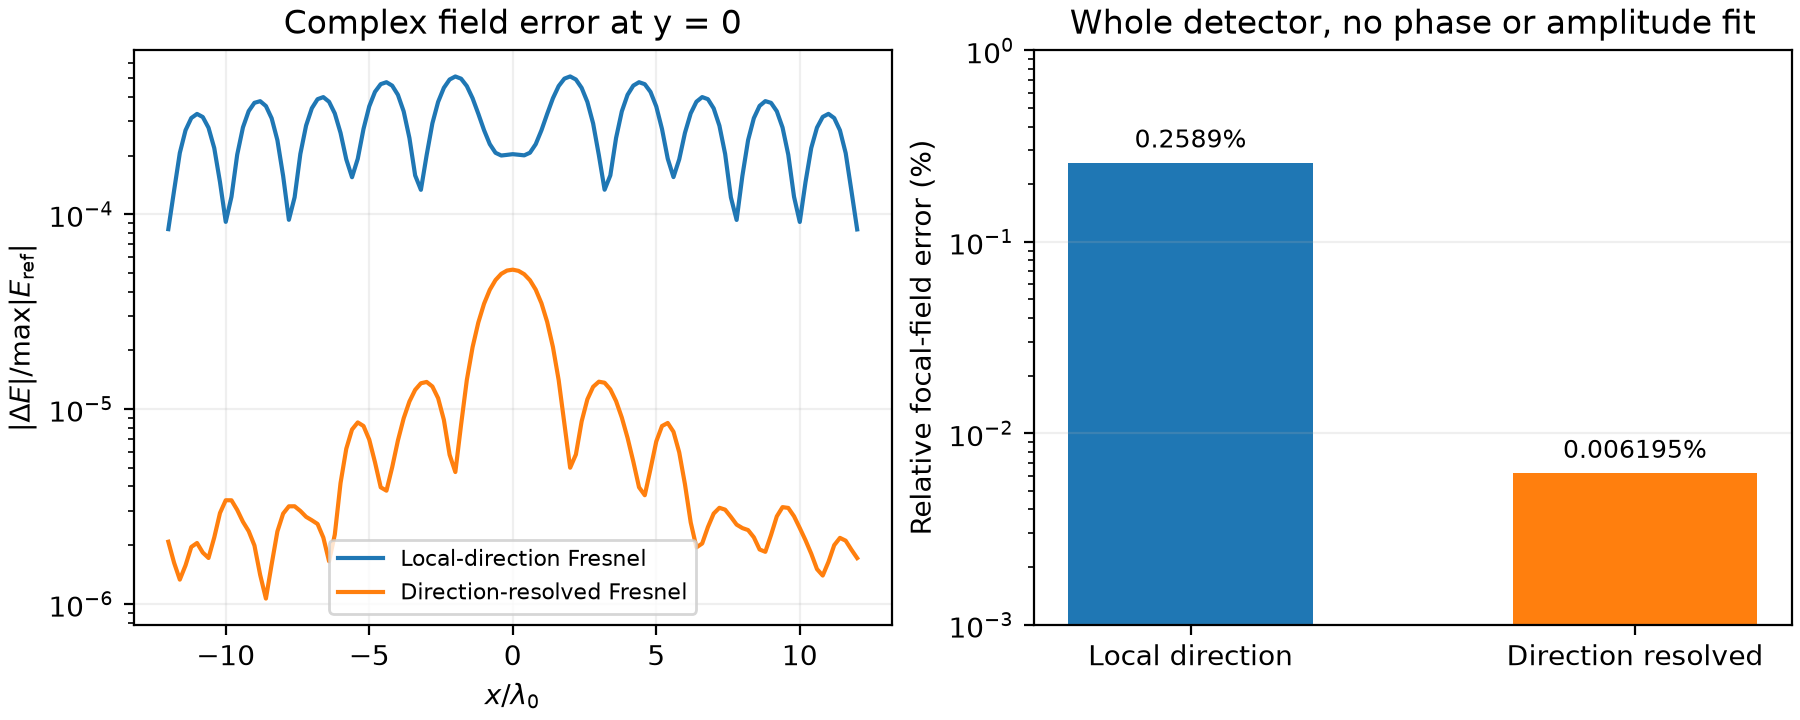
\includegraphics[width=\linewidth]{fresnel_comparison}
 \caption{Fresnel-only comparison at $280^2$ spatial samples. Left: absolute
 complex electric-field error on the focal-plane line $y=0$, normalized by the
 reference peak field. Right: relative $L^2$ errors over the whole detector.
 The same exact single-pass reference and unadjusted complex fields are used.}
 \label{fig:comparison}
\end{figure}

The refined angular calculation used 18 nodes per direction coordinate at
entrance. At exit it used a central patch $[-0.3,0.3]^2$ with 18 nodes per axis
and eight outer patches with 6 nodes per axis. The modal selection used a
relative amplitude threshold $10^{-7}$ and a direction-coordinate cap
$|d_1|,|d_2|\le0.65$. The measured omitted modal $L^2$ fractions were
$1.63\times10^{-6}$ at entrance and $3.02\times10^{-7}$ at exit; these fractions
are diagnostics, not bounds on the final focal error.

Increasing the central angular resolution from 12 to 18 nodes, the outer
resolution from 4 to 6 nodes, and tightening the modal threshold from $10^{-6}$
to $10^{-7}$ changed the complex focal field by $1.22\times10^{-5}$.
The error norm against the reference remained near $6.2\times10^{-5}$.
At sampled entrance points the refined interpolated trace differed from a
direct spectral sum by $5.87\times10^{-7}$; at the sampled exit points,
including dark and critical regions, the discrepancy was $3.09\times10^{-3}$.
Thus the focal improvement is measured directly, but uniform convergence of
the surface response has not been established. A single angular patch covering
the full exit range was rejected because its sampled direct-sum discrepancy
was about one percent.

The recorded refined direction-resolved run took 185.7~s for interface
application, direct-sum audits, reconstruction and detector evaluation, after
29.8~s of shared transport setup. Input-spectrum preparation and initial trace
evaluation were not separately timed in this run. These values are partial
single-run timings of a validation prototype on an Apple M4 with single-thread
BLAS settings, not a complete production throughput comparison.

Against the full Lorenz--Mie field, the same direction-resolved Fresnel result
has error $0.41020\%$. The exact single-pass reference itself differs from full
Mie by $0.41016\%$. Scattering branches omitted by the one-way composition
therefore dominate that comparison. Raising the accuracy of the one-pass
interface operator cannot supply those branches.

\subsection{Performance without changing the angular discretization}

A subsequent implementation audit held the $280^2$ spatial charts, angular
nodes, modal cutoff and Fresnel coefficients fixed. The optimized computation
retained the same 20,665 entrance and 47,142 exit modes. Its focal electric and
magnetic fields differed from the original implementation by approximately
$5.6\times10^{-15}$ in relative norm; the largest relative difference among
the complete entrance and exit electric and magnetic traces was
$1.2\times10^{-14}$. The focal electric-field error against the exact
single-pass reference remained $0.00619492147\%$.

The principal rearrangement is to build the scalar transport separation over
the occupied longitudinal bandwidth of each angular patch. For a patch with
$k_z\in[k_{z,\min},k_{z,\max}]$, choose
$k_c=(k_{z,\min}+k_{z,\max})/2$ and use
\begin{equation}
 e^{i k_z h}=e^{i k_c h}e^{i(k_z-k_c)h}.
\end{equation}
The original modal phases remain intact. The same Chebyshev--Bessel expansion
then requires fewer terms: 85 to 52 at entrance, 119 to 38 in the central exit
patch, and 119 to 71--72 in the outer exit patches. The scalar kernel tail
budget was tightened from $10^{-10}$ to $10^{-12}$.

Additional savings come from evaluating Bessel functions only at exactly
distinct active arguments, applying the Fresnel symbol directly without
constructing a temporary $2\times6$ matrix or an unused reflected field, and
omitting summed incident traces that ordinary direction-resolved Fresnel does
not use. Such traces remain necessary for the local-direction method, direct
audits and the implemented higher-order corrections. Compact spectral storage,
contiguous spatial FFT axes, omission of exactly zero polarization channels,
and a bounded cache of angular-patch plans reduce memory traffic. The final
measurement used two FFT workers in the optimized synthesis and approximately
469~MiB of cached patch plans.

\begin{table}[htbp]
\centering
\caption{First-evaluation numerical timings on an Apple M4, with the same
angular discretization. Direct-sum audits, reference comparisons, imports and
artifact I/O are excluded from both paths.}
\begin{tabular}{lrr}
\toprule
Stage & Original (s) & Optimized (s)\\
\midrule
Shared transport setup & 30.00 & 2.30\\
Source preparation and required incident trace & 40.51 & 0.043\\
Interfaces, reconstruction and detector & 146.96 & 38.31\\
\midrule
Sum & 217.48 & 40.65\\
\bottomrule
\end{tabular}
\end{table}

The sum decreased by a factor of 5.35. A second evaluation of the same input,
with geometry and source already prepared, took 159.64~s for the original path
and 38.65~s for the optimized path. These are serial workstation measurements,
not a statistical throughput study or a comparison with a matched BEM solve.
The original timings precede the shared Bessel-argument setup optimization;
that change also benefits the original path when it is rerun. These prototype timings are retained as historical measurements in the
stored performance records. The supported implementation now lives in
\texttt{vecdiff\_general.propagation}. The same compact bandwidth plans,
fused vector response and bounded cache are used there. They preserve the
measured discretization and physical-model errors; they do not establish
uniform convergence near angular branch boundaries.

\subsection{Implementation status and reproducibility}

The public implementation separates homogeneous propagation
(\texttt{homogeneous.py}), surface transfer (\texttt{surface\_transfer.py}),
surface interaction (\texttt{surface\_interaction.py}), and path composition
(\texttt{pipeline.py}). \texttt{DirectionResolvedFresnel} is the default
transmission model of \texttt{PropagationPipeline}. The outgoing reconstruction
uses surface equivalence; the separate least-squares inverse remains available
for pure-transfer checks. Mie, Debye and BEM references live in
\texttt{propagation/references} and are not used in the candidate calculation.

The original experiments used a historical higher-order response module from
revision \texttt{5d395e1}; order zero used ordinary Fresnel coefficients.
That experimental harness and the former local-direction pipeline have been
retired. The stored records preserve their comparison data:
\begin{quote}\small\ttfamily
 validation/reference\_data/focal\_pipeline.json\\
 validation/reference\_data/focal\_spectral\_N280\_a18\_c1e-07\_t3.json
\end{quote}
Corresponding arrays contain the complex focal fields. The suffix
\texttt{t3} denotes the three-interval angular partition, not curvature order;
the ordinary Fresnel row has \texttt{order=0}.

From the repository root, the current Fresnel-only pipeline is checked against
those saved fields and the independently computed Debye $p=1$ reference by
\begin{quote}\small
\begin{verbatim}
OPENBLAS_NUM_THREADS=1 OMP_NUM_THREADS=2 \
VECLIB_MAXIMUM_THREADS=1 .venv/bin/python \
validation/pipeline_regression.py
\end{verbatim}
\end{quote}
The command writes \texttt{validation/reference\_data/pipeline\_regression.json},
including end-to-end solve and focal evaluation times. The reference arrays
are loaded only after the candidate solution has been computed. This checks
reproducibility against frozen references; it does not regenerate them.
Unit tests separately compare the core against direct modal synthesis,
planar boundary conditions, and pure transfer of analytical and BEM fields.
Finite material edges, stops, incident evanescent modes in Q, and returning
branches remain outside the supported curved-surface pipeline.

\begin{thebibliography}{10}
\bibitem{Weyl1919}
 H. Weyl, ``Ausbreitung elektromagnetischer Wellen über einem ebenen Leiter,''
 \emph{Annalen der Physik} \textbf{365}, 481--500 (1919).
 \href{https://doi.org/10.1002/andp.19193652104}{doi:10.1002/andp.19193652104}.
\bibitem{Schelkunoff1936}
 S. A. Schelkunoff, ``Some equivalence theorems of electromagnetics and their
 application to radiation problems,'' \emph{Bell System Technical Journal}
 \textbf{15}, 92--112 (1936).
 \href{https://doi.org/10.1002/j.1538-7305.1936.tb00720.x}{doi:10.1002/j.1538-7305.1936.tb00720.x}.
\bibitem{StrattonChu1939}
 J. A. Stratton and L. J. Chu, ``Diffraction theory of electromagnetic waves,''
 \emph{Physical Review} \textbf{56}, 99--107 (1939).
 \href{https://doi.org/10.1103/PhysRev.56.99}{doi:10.1103/PhysRev.56.99}.
\bibitem{Esmer2011}
 G. B. Esmer, L. Onural and H. M. Ozaktas, ``Exact diffraction calculation from
 fields specified over arbitrary curved surfaces,'' \emph{Optics
 Communications} \textbf{284}, 5537--5548 (2011).
 \href{https://doi.org/10.1016/j.optcom.2011.07.040}{doi:10.1016/j.optcom.2011.07.040}.
\bibitem{Tessmer2015a}
 M. Tessmer and H. Gross, ``Generalized propagation of light through optical
 systems. I. Mathematical basics,'' \emph{Journal of the Optical Society of
 America A} \textbf{32}, 258--266 (2015).
 \href{https://doi.org/10.1364/JOSAA.32.000258}{doi:10.1364/JOSAA.32.000258}.
\bibitem{Tessmer2015b}
 M. Tessmer and H. Gross, ``Generalized propagation of light through optical
 systems. II. Numerical implications,'' \emph{Journal of the Optical Society
 of America A} \textbf{32}, 2276--2285 (2015).
 \href{https://doi.org/10.1364/JOSAA.32.002276}{doi:10.1364/JOSAA.32.002276}.
\bibitem{Lasso2013}
 W. Lasso, M. Navas, L. A\~nez, R. Urdaneta, L. D\'iaz and C. O. Torres,
 ``Diffraction operators in paraxial approach,'' \emph{Education and Training
 in Optics and Photonics}, paper EWP5 (2013).
 \href{https://opg.optica.org/abstract.cfm?uri=etop-2013-EWP5}{Optica proceedings record}.
\bibitem{PellatFinet1994}
 P. Pellat-Finet, ``Fresnel diffraction and the fractional-order Fourier
 transform,'' \emph{Optics Letters} \textbf{19}, 1388--1390 (1994).
 \href{https://doi.org/10.1364/OL.19.001388}{doi:10.1364/OL.19.001388}.
\bibitem{Barnett2019}
 A. H. Barnett, J. Magland and L. af Klinteberg, ``A parallel nonuniform fast
 Fourier transform library based on an `exponential of semicircle' kernel,''
 \emph{SIAM Journal on Scientific Computing} \textbf{41}, C479--C504 (2019).
 \href{https://doi.org/10.1137/18M120885X}{doi:10.1137/18M120885X}.
\end{thebibliography}
\end{document}
